\section{Практична частина}
\setlength{\parindent}{4em}
\subsection{Визначення постійної дифракційної гратки і кількості штрихів на мм}

\begin{figure}[ht]

\centering

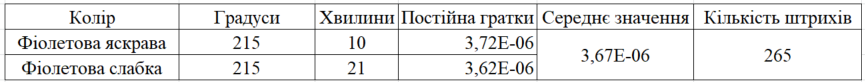
\includegraphics[width=1\linewidth]{Pics/tabl1.png}

\label{table1}

\end{figure}

\subsection{Визначення довжин хвиль спекту ртуті}

\begin{figure}[ht]

\centering

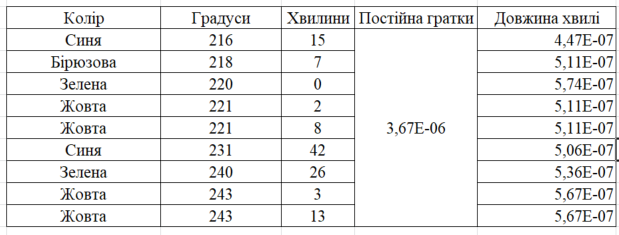
\includegraphics[width=1\linewidth]{Pics/tabl2.png}

\label{table1}

\end{figure}
\newpage

\subsection{Визначення кутової дисперсії}
\subsubsection{Для першого порядку}
\begin{figure}[ht]

\centering

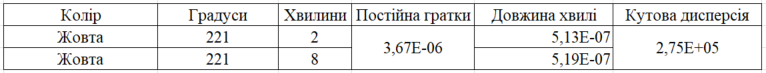
\includegraphics[width=1\linewidth]{Pics/tabl3.png}

\label{table1}

\end{figure}
\subsubsection{Для другого порядку}

\begin{figure}[ht]

\centering

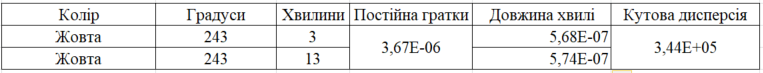
\includegraphics[width=1\linewidth]{Pics/tabl4.png}

\label{table1}

\end{figure}
